\documentclass[dvipsnames]{article}
\usepackage[utf8]{inputenc}
\usepackage{graphicx, amsmath, amssymb}
\usepackage[mode=buildnew]{standalone}
\usepackage{hyperref}
\usepackage{float}
\graphicspath{ {./images/} }
\usepackage[dvipsnames]{xcolor}
\usepackage{titlesec}
\usepackage{tikz}
\usepackage[margin=1in]{geometry}
\usepackage{multicol}
\usetikzlibrary{arrows.meta, positioning}
\DeclareMathOperator*{\KL}{KL}
\newcommand\encircle[1]{%
  \tikz[baseline=(X.base)] 
    \node (X) [draw, shape=circle, inner sep=0] {\strut #1};}
\title{Variational Autoencoder}
\author{Sumit Singh}
\date{\today}

\begin{document}

\maketitle




%******************************************************
\section{Introduction}
%******************************************************


%******************************************************
\section{(Deterministic) Autoencoder}
%******************************************************
\textit{What is an Autoencoder?} \\
An autoencoder is a special type of feed-forward Neural Network with an encoder \& decoder architecture trained by backpropagation to minimize reconstruction loss. It consists of two parts:
\begin{itemize}
    \item An \textbf{Encoder} network $E(x)$ that deterministically transforms the input $x$ into a latent vector representation $z$
    \item A \textbf{Decoder} network $D(z)$ that maps the latent vector back to the input space, attempting to reconstruct $x$
\end{itemize}
\begin{figure}[H]
    \centering
    \includegraphics[width=0.95\linewidth]{GenAI/Images/15DeterministicAutoEncoderI.jpg}
    \caption{Deterministic Autoencoder}
    \label{fig:deterministicAutoencoder}
\end{figure}
Autoencoders, especially deep ones, can model non-linear relationships because they are neural networks with non-linear activation functions. An autoencoder takes $x$ and produces $\hat{x}$ through a bottleneck. The networks are trained so that $\hat{x}$ is as close as possible to the original $x$ (for example, minimizing $||x-\hat{x}||^2$. Through the many layers, the encoder gradually compresses and transforms the input through a hierarchy of features; likewise the decoder reconstructs through layers.
\subsection{PCA and Autoencoder (Linear Encoders and Decoders)}
A linear autoencoder: single hidden layer, no activation function/linear encoder \& decoder, MSE Loss, bottleneck ($z$) dimension $<$ input dimension of $x$, learns the same subspace as PCA. 
\begin{figure}[H]
    \centering
    \includegraphics[width=0.5\linewidth]{GenAI/Images/15DetermininisticAE2.jpg}
    \caption{Autoencoder}
    \label{fig:placeholder}
\end{figure}
The linear/simple autoencoder is merely a matrix multiplication.
\begin{align*}
    z &= U^T x \quad  x  \in \mathbb{R}^{d \times 1}  \quad z \in \mathbb{R}^{p \times 1} \quad p < d \\
    \hat{x} &= Uz \quad  \hat{x}  \in \mathbb{R}^{d \times 1}
\end{align*}
In PCA/SVD:
\begin{align*}
    &|| \hat{x} - U^TUx||^2 \\
    & \text{s.t. } U^TU = I, \text{ and rank}(U)=k.ST
\end{align*} 
We want $x$ to be similar to $\hat{x}$ in the autoencoder as well. We want to go through the bottleneck and regenerate the input. The difference between PCA\slash SVA, and a simple linear autoencoder is that there is no constraint of $UU^T = I$. So the solution will not be identical to PCA\slash SVA but it is going to span the same space as the basis. \\
\subsection{Autoencoder}
The encoder\slash decoder is not merely a matrix multiplication. There are many layers; there is non-linearity between the layers. If there are many layers, then it is a deep autoencoder. \\
There are ``over-complete" autoencoders as well, where the latent vector has a higher dimension than the input\slash output dimension. It is used for denoising. \\


\textcolor{red}{\textit{ How is autoencoder used to denoise images with Gaussian white noise?}} \\

\textcolor{blue}{\textit{ First, white noise will be added to regular images and used as input and the image as the output, Let $f$ be the autoencoder, $x$ and image, and $w$ be white noise. The autoencoder will be trained to convert $f(x+w)$ to $x$.}} \\
\textcolor{blue}{\textit{Then, the trained autoencoder can be used to remove white noise from unseen images.}} \\









%******************************************************
\section{Variational Autoencoder vs Deterministic Autoencoder}
%******************************************************
\begin{figure}[H]
    \centering
    \includegraphics[width=0.95\linewidth]{GenAI/Images/15VAE1.jpg}
    \caption{Variational Autoencoder}
    \label{fig:placeholder}
\end{figure}
The difference between a variational autoencoder and a deterministic autoencoder is that $z$ comes from a certain distribution. You pass $x$ to the model; you want to reconstruct $x$, subject to the constraint that $z$ is Gaussian (say). If $z$ is Gaussian, then you can use the Decoder as a Generative model. We can generate a Gaussian random variable, pass it through the decoder, and generate values of $x$. \\
Suppose we first train on the CIFAR10 dataset (horses, cats, dogs, ships, trucks, cars, airplanes, etc.).  After training, we take the decoder out. Then, we sample from the Gaussian ($z$ is Gaussian) and pass it through the decoder. The output should be similar to the objects in CIFAR10. Say there is an image of a horse that is not present in CIFAR10 or anywhere else. Now, we have a transformer that can generate a horse, a car, a cat, or a truck from a Gaussian. This can be used as a Generative model. \\   



Variational Autoencoders are based on Variational Inference. 














%******************************************************
\section{Variational Inference}
%******************************************************
 Variational Inference is a powerful technique in Bayesian Statistics and Machine Learning for approximating complex posterior distributions. In Bayesian statistics:
 \begin{itemize}
     \item  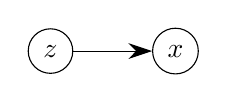
\begin{tikzpicture}[
  node/.style = {circle, draw, minimum size=0.5cm},
  >={Stealth[length=3mm, width=2mm]}  % arrow style
]
  % Define nodes
  \node[node] (z) {$z$};
  \node[node] (x) [right=1cm of z] {$x$};

  % Draw directed edge from z to x
  \draw[->] (z) -- (x);

\end{tikzpicture}
     \item $p(z|x)$: Posterior
     \item $z$: Latent (hidden) Variable
     \item $x$: Observed Data. Likelihood or observation model, relating data to latent variables.
     \item Given the observation ($x$), what is the code ($z$) that generated this observation?
     \item \begin{align*}
         p(z|x) &= \frac{p(x|z) p(z)}{p(x)} \\
         p(x) &= \int_z p(x|z) p(z) \\
         p(z|x) &=  \frac{p(x|z) p(z)}{\int_z p(x|z) p(z) }
     \end{align*}
     \item $p(x) = \int_z p(x|z) p(z)$ is difficult to compute. It is \textit{intractable}.
     \item $p(x|z)$ is easy to compute. $p(z)$ is the prior.
 \end{itemize}
 
\textit{What are latent variables in Variational Inference?} \\
Latent variables are hidden (unobserved) variables. Let us assume that $x = x_{1:n}$ represents observations and $z = z_{1:m}$ represents hidden variables. 
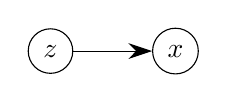
\begin{tikzpicture}[
  node/.style = {circle, draw, minimum size=0.5cm},
  >={Stealth[length=3mm, width=2mm]}  % arrow style
]
  % Define nodes
  \node[node] (z) {$z$};
  \node[node] (x) [right=1cm of z] {$x$};

  % Draw directed edge from z to x
  \draw[->] (z) -- (x);

\end{tikzpicture}
In probabilistic models, latent (hidden/unobserved) variables are 
variables that we do not directly observe (often denoted as $z$), but we assume they influence the observed data $x$. You do not observe $z$. You observe $x$. $x$ is governed by the hidden variable $z$. Hidden/Latent variables represent the underlying structure or ``explanatory factors" of the data. Given the observation, what is the code that generated this observation? That is the case with regression, classification, and topic modeling.  Factor Analysis, Hidden Markov Models (HMM), Latent Dirichlet Allocation (LDA), and Structural Equation Modeling (SEM) are models that use latent variables. \\ 
\textbf{Generative Model Perspective}: The generative model is typically something like:
\begin{align*}
    p_\theta (x,z) = p_\theta(x|z) \cdot p_\theta (z)
\end{align*}
Here, $p_\theta (z)$ is the prior over the latent variable, and $p_\theta (x|z)$ is how we generate data given $z$. \\


The \textbf{marginal likelihood} of the data (what we really care about) is:
\begin{align*}
    p_\theta(x) = \int p_\theta (x,z) dz = \int_z p_\theta (x|z) p_\theta (z) dz 
\end{align*}
Usually, this integral is intractable for complex models. If $z$ is high dimensional, $p_\theta(x) = \int_z p_\theta (x|z) p_\theta (z) dz$ is intractable. That is one of the main obstacles in Graphical Models.
\begin{align*}
    \int \int \int \int \int \int \cdot \cdot \cdot \cdot \cdot dz
\end{align*}


\textbf{Posterior over Latent Variables ($p_\theta (z|x)$)} : What we really want in Bayesian inference is the posterior $p_\theta(z|x)$  -- how latent variables $z$ are distributed given the observed data $x$. But it is often intractable because it involves the marginal likelihood ($p_\theta (x)$) in the denominator.  
\begin{align*}
    p_\theta (z|x) = \frac{p_\theta (x|z) \cdot p_\theta (z)}{p_\theta (x)}
\end{align*}
$p(x|z)$ is easy to compute. $p_\theta (z)$ is the prior. $p_\theta (x)$, the marginal likelihood is hard to compute.
\\
In Bayesian Statistics, we often want to compute the posterior. The substantial literature on graphical models or Bayesian Statistics focuses on approximating this marginal likelihood $p_\theta (x)$, which is an intractable quantity. There are many different techniques.
\begin{itemize}
    \item One line of technique is sampling-based methods, such as Monte Carlo Methods. Importance Sampling, MCMC Pseudo-Marginal / Particle MCMC, and Nested Sampling are different Monte Carlo Methods. Both Gibbs sampling and Metropolis Hastings are part of the MCMC category of approximate Bayesian inference. Gibbs sampling is a special case of Metropolis-Hastings. 
    \item Another set of techniques is Variational Inference
\end{itemize}
So instead, we approximate the true posterior with a more tractable distribution $q_\phi (z|x)$. This is where variational inference comes in. Variational Inference, in principle, means allowing us to transform this intractable quantity, $p_\theta (z|x)$, into an optimization problem. It is done by assuming that another distribution exists, which is tractable. Find the parameter of that one such that it is quite close to $p_\theta (z|x)$. If it is close to $p_\theta (z|x)$, I use it as a surrogate.\\
Assume that there is a $q(z)$. $q$ comes from a well behaved family (e.g., Gaussian). It is parameterized by $\phi$: $q_\phi (z|x)$. \\
We want to minimize the KL Divergence of this $q$ with my posterior:
\begin{align*}
    min \quad \KL_{\phi} (q_\phi (z|x) || p_\theta(z|x))
\end{align*}
If I can minimize this Kullback-Leibler Divergence  and find appropriate $\phi$s, the $q_\phi (z)$ is close to my posterior $p(z|x)$, and $q_\phi(z)$ is well behaved (it is from Gaussian). Hence, we will use $q_\phi(z)$ instead of $p_\theta (z|x)$. $\phi$ depends on $x$, it is a function of $x$. \\
It is not easy to minimize the Kullback-Leibler divergence:
\begin{align*}
    min \quad \KL_\phi (q_\phi (z|x) || p_\theta(z|x) )
\end{align*}
This is so because the Kullback-Leibler divergence depends on a quantity that is unknown : $p_\theta (z|x)$. The problem that we started with was: we do not know what's $p_\theta (z|x)$ is? Variational Inference is a way to get around this.\\ 
\subsection{KL Divergence}
Kullback-Leibler divergence measures the similarity between two distributions. It is the expected \textbf{excess surprise} from using $Q$ as a model instead of $P$ when the actual distribution is $P$ \\
It comes from Information Theory. If $x$ is an event, the Information $I$ of an event $x$ is given by:
\begin{align*}
    I = - log(p(x))
\end{align*}
Higher Probability $\implies$ Lower Information. The information: ``the sun is going to rise in the east tomorrow" is a sure (very high probability) event with absolutely no information. While the information: ``There is going to be a meteor shower on a certain night" is a low probability event with high information. \\
\begin{align*}
    Entropy: \quad H = \mathbb{E}[I] = - \sum p(x) \cdot log(p(x))
\end{align*}
\begin{align*}
    Cross-Entropy: \quad H(X,Y) &= \sum_{x \in X} Surprise(Y=x) \cdot P(X=x) \\
    &= \sum_{x \in X} \frac{1}{ log P(Y=x)} \cdot P(X=x)
\end{align*}
\begin{align*}
    D_{KL} (P||Q) &= \sum_{x \in X} [Surprise(Q=x) - Surprise(P=x)] \cdot P(P=x) \\
    &= \sum_{x \in X}  log \frac{P(P=x)}{P(Q=x)}  \cdot P(P=x)
\end{align*}
\begin{align*}
    D_{KL} (P||Q) = \sum_x P(x) \cdot log \frac{P(x)}{Q(x)} = \int_{- \infty}^{\infty} p(x) \cdot ln \frac{p(x)}{q(x)}
\end{align*}
\begin{align*}
    D_{KL}(Q||P) = \sum_x Q(x) \cdot log \frac{Q(x)}{P(x)} = \int_{- \infty}^{\infty} q(x) \cdot ln \frac{q(x)}{p(x)}
\end{align*}
\begin{align*}
    D_{KL} (P||Q) \neq D_{KL} (Q||P)
\end{align*}
\begin{align*}
    H(P) - H(Q) &= [-\sum p(x) log(p(x)] - [-\sum q(x) log(q(x))] \\
    & \neq [-\sum q(x) log(p(x)] - [-\sum q(x) log(q(x))] \\
    \implies H(P) - H(Q)  & \neq D_{KL} (Q||P)
\end{align*}

\begin{align*}
    KL(Q||P) &= - \sum q(x) \times log\big(p(x)\big) - \bigg(-\sum q(x) \times log\big(q(x)\big) \bigg) \\
    &= \sum q(x) \times log\big(q(x)\big) - \sum q(x) \times log\big(p(x)\big) \\
    &= \sum q(x) log \frac{q(x)}{p(x)} \\
    &= - \sum q(x) log \frac{p(x)}{q(x)}
\end{align*}
In KL divergence, you compute the divergence with respect to a certain probability distribution. KL divergence tells you the information loss if you want to transform it to another distribution. That is why it is a measure of similarity between two distributions. $D_{KL}(P||Q) \geq 0$ \& $D_{KL}(P||Q) \neq D_{KL}(Q||P)$. KL divergence is not symmetric. It is not the distance. It is the divergence.
\subsubsection{Kullback-Leibler Divergence of Bernouli}
Let $X \sim Bern(p_\alpha)$ and  $Y \sim Bern(p_\beta)$. What is the KL Divergence between them?
\begin{align*}
    D_{KL}(X,Y) &= \sum_x [log \frac{1}{P(Y=x)} - log \frac{1}{P(X=x)}] \cdot P(X=x) \\
    &= [log \frac{1}{P(Y=1)} - log \frac{1}{P(X=1)}] \cdot P(X=1) \\
    &+ [log \frac{1}{P(Y=0)} - log \frac{1}{P(X=0)} ] \cdot P(X=0) \\
    &= [log \frac{1}{p_b} - log \frac{1}{p_a}] \cdot p_a + [log \frac{1}{1-p_b} - log \frac{1}{1-p_a}] \cdot (1-p_a) \\
    &=  p_a log \frac{p_a}{p_b} + (1-p_a) log \frac{1-p_a}{1-p_b} \\
    D_{KL}(0.8||0.4) &= 0.8 log \frac{0.8}{0.4} + 0.2 log \frac{0.2}{0.6} \\
    &=  0.8 log 2 + 0.2 log\frac{1}{3} \\
    &= 0.8 \times 0.6931 + 0.2 \times (-1.0986) \\
    &= 0.5545 - 0.2197 \\
    &= 0.3348 \\
    D_{KL}(0.4||0.8) &= 0.4 log \frac{0.4}{0.8} + 0.6 log \frac{0.6}{0.2} \\
    &= 0.4 log(0.5) + 0.6 log 3 \\
    &= 0.4 \times (-0.6931) + 0.6 \times 1.0986 \\
    &= -0.2772 + 0.6592 \\
    &= 0.3820
\end{align*}

\textit{How does Variational Inference work with Latent Variables?} 
\begin{itemize}
    \item \textbf{Approximate Posterior (Variational Distribution)}
    \begin{itemize}
        \item We pick a parametric family for $q_\phi (z|x)$ (e.g., a Gaussian) that's easier to work with
        \item The goal is to make $q_\phi (z|x)$ as close as possible to the true posterior $p_\theta (z|x)$. The closeness is measured using KL divergence.
    \end{itemize}
    \item \textbf{Evidence Lower Bound (ELBO)}
    \begin{itemize}
        \item Instead of maximizing the intractable log-likelihood $log$ $p_\theta (x)$ directly, we maximize a lower bound called the ELBO
        \item The ELBO is:
        \begin{align*}
            \mathbb{E}_{q_\phi (z|x)} [log p_\theta (x|z)] - KL(q_\phi (z|x) || p_\theta (z))
        \end{align*}
    \end{itemize}
    \item \textbf{Reparameterization Trick}
\end{itemize}
In this scenario: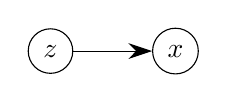
\begin{tikzpicture}[
  node/.style = {circle, draw, minimum size=0.5cm},
  >={Stealth[length=3mm, width=2mm]}  % arrow style
]
  % Define nodes
  \node[node] (z) {$z$};
  \node[node] (x) [right=1cm of z] {$x$};

  % Draw directed edge from z to x
  \draw[->] (z) -- (x);

\end{tikzpicture}
We have a simple graphical model. We want to 
\begin{align*}
 min \quad \KL_\phi (q_\phi (z|x) || p_\theta(z|x) )    
\end{align*}
When $p$ is intractable, we cannot do it directly because $p(z|x)$ is unknown.
\begin{align*}
    KL(q(z)||p(z|x)) &= - \int q(z) \ log \frac{p(z|x)}{q(z)} dz \\
    p(z|x) &= \frac{p(x|z) \cdot p(z)}{p(x)} = \frac{p(z,x)}{p(x)} \\
    \implies KL(q(z) || p(z|x) &= - \int q(z) \ log \bigg[  \frac{p(z|x)}{q(z)} \cdot \frac{1}{p(x)}  \bigg]dz \\
    &= - \int q(z) \bigg[  log \frac{p(z|x)}{q(z)} - log(p(x) \bigg] dz \\
    &= - \int q(z) \ log \frac{p(z|x)}{q(z)} + \int_q q(z) \ log(p(x)) dz \\
    &= - \int q(z) \ log \frac{p(z|x)}{q(z)} +  log(p(x) \int_q q(z) dz \\
    &= - \int q(z) \ log \frac{p(z|x)}{q(z)} +  log(p(x) \\
    \implies min \quad \KL_\phi (q_\phi (z|x) || p_\theta(z|x) )  &= \min_\phi \bigg[ - \int q(z) \ log \frac{p(z|x)}{q(z)} +  log(p(x) \bigg] \\
     &= \max_\phi \int_q q(z) log \frac{p(z,x)}{q(z)} dz \\
     ELBO &= \max_\phi \int_q q(z) log \frac{p(z,x)}{q(z)} dz 
 \end{align*}
ELBO: Evidence Lower Bound / Variational Lower Bound. In Variational Inference, you start by minimizing the KL divergence to create a tractable distribution that is similar to an intractable distribution. The whole idea is to compute the ELBO. Instead of minimizing KL divergence, maximize the ELBO. ELBO is tractable. It does not depend on the unknowns $z$ or $x$. It depends on $p(z,x)$, the joint distribution, which is tractable and $q(z)$, the well behaved distribution that we have chosen (as Gaussian). \\
\textit{Why do we call the ELBO a lower bound?}
\begin{align*}
    log(p(x)) &= \KL_\phi (q_\phi(z|x) || p_\theta(z|x)) + \int q(z) log \frac{p(z,x)}{q(z)} \\
     \mathcal{L} &= \int q(z) log \frac{p(z.x)}{q(z)} \\
     &= Lower \ Bound \\
     Log(p(x)) &= Constant
\end{align*}



\begin{multicols}{2}
\documentclass[tikz,border=5pt]{standalone}
\begin{document}
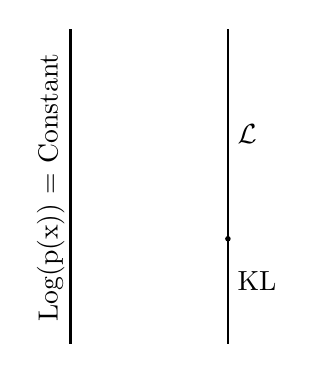
\begin{tikzpicture}

  % length of segment
  \def\L{4}  % change as needed

  % First full vertical line
  \draw[thick] (0,0) -- (0,\L);

  % Second vertical line divided into two equal parts
  % We'll draw two segments, each of length L/2
  \draw[thick] (2,0) -- (2,\L/2);
  \draw[thick] (2,\L/2) -- (2,\L);

  % optionally, mark the division point
  \fill (2, \L/3) circle(1pt);

  % optionally, add labels
  \node[rotate=90,left] at (-0.25, \L/1.05) {Log(p(x)) = Constant};
  \node[right] at (2, \L/1.5) {$\mathcal{L}$  };
  \node[right] at (2, \L/5) {KL};

\end{tikzpicture}
\end{document}

\columnbreak

$\mathcal{L}$ is lower bound of $log(p(x))$, the log probability, the likelihood of the data. You have computed the lower bound of your likelihood. When you maximize the lower bound, you push the likelihood up. 
\begin{align*}
    \mathcal{L} &= \int q(z) log \frac{p(z,x)}{q(z)}
\end{align*}
\end{multicols}
$\mathcal{L}$ is tractable.
\begin{align*}
    \mathcal{L} &= \int q(z) log \frac{p(z,x)}{q(z)} \\
    &= \int q(z) log \frac{p(x|z) p(z)}{q(z)} \\
    &= \int  q(z) log (p(x|z)) + \int q(z) log \frac{p(z)}{q(z)} \\
    \int  q(z) log (p(x|z))  &= \mathbb{E}[log(p(x|z))] \\
    &= \mathbb{E}[\text{Log Likelihood of my observation}] \\
    \int q(z) log \frac{p(z)}{q(z)}  &= -KL(q(z)||p(z)) \\
    \implies \mathcal{L} &= \mathbb{E}[log(p(x|z))] - KL(q(z)||p(z)) \\
    maximize \ \mathcal{L} &\implies min \ [KL(q(z)||p(z))]
\end{align*}
This $KL(q(z)||p(z))$ is tractable. [\textit{Is $KL(q(z)||p(z|x) )$ tractable?}] $q$ is from a well behaved distribution that we have chosen. $\mathbb{E}[log(p(x|z))]$ is the likelihood of our data, and we maximize the likelihood of our data. The idea here is that in the \encircle{$z$} $ \rightarrow $ \encircle{$x$}, graphical model, we generate $x$ given $z$. (?) $p(x|z)$ and I hope to be able to compute this posterior, $p(z|x)$. We decided that we approximate $p(z|x)$ by some $q_\phi(z)$, $q$ parametrized by $\phi$.
\begin{multicols}{2}
\begin{figure}[H]
    \centering
    \includegraphics[width=0.75\linewidth]{GenAI/Images/15VAE2.jpg}
    \caption{VAE}
    \label{fig:VAEOF}
\end{figure}

\columnbreak
In the encoder, the input is $x$ and the output is $z$. The decoder takes $z$ and outputs $\hat{x}$ to reproduce$x$. The idea is to approximate the encoder and the decoder. Approximating the encoder with $q_\phi$ and approximating the decoder with $p_\theta$. These two neural networks are going to be functions that approximate these two probabilities: ($q_\phi(z|x)$ and $p_\theta(x|z)$).


\end{multicols}
\begin{align*}
\mathcal{L} &= \mathbb{E}[log(p(x|z))] - KL(q(z)||p(z)) \\
\end{align*}
To train the model, we have to maximize $\mathcal{L}$. $\mathcal{L}$ has two parts: 
\begin{itemize}
    \item $q$ comes from a well behaved distribution of my choice. I chose $q$ to be Gaussian. I have to minimize the KL Divergence between Gaussian ($q$) and $p$.
    \item $\mathbb{E} [log(p(x|z))]$: Maximize the likelihood. You can directly maximize the likelihood or make some assumptions. If your assumption is that $p$ is Gaussian, then maximizing the likelihood is the same as minimizing the mean squared error. If your assumption is that $p$ is Bernoulli, then it will be the same as minimizing cross-entropy. 
\end{itemize}
My objective function here (~\ref{fig:VAEOF}) would be $\mathbb{E}[log(p(x|z))]$ with the assumption that it is Gaussian. I have to minimize the reconstruction $|x - \hat{x}|$ and I have to make sure that $q$ is Gaussian. 
\begin{align*}
    |x-\hat{x}| + KL(q(z)||\mathcal{N}( \quad )  )
\end{align*}
In a deterministic autoencoder, the only constraint is to minimize $|x-\hat{x}|$ (the reconstruction loss). Now, in the VAE, we have an additional constraint added to our objective function. This additional term ensures that $z$ is Gaussian. Reconstruct the points and ensure that $z$, the latent variable (vector), is Gaussian, as this will constitute a variational autoencoder. This additional term changes it from a deterministic autoencoder to a variational autoencoder. \\
\section{Re-parameterization Trick}
The problem in practice in the above model is that: $z$ is stochastic. You cannot pass gradient (for backpropagation) through a stochastic layer. If it is not deterministic, you cannot take derivatives. Backpropagation will not compute an estimate of the derivative through a random node.\\
To handle this: \textbf{Re-parameterization Trick}: entangle the stochasticity of the problem with the parameters. Gaussian is stochastic, but it comes from a distribution that can have deterministic parameters: $\mu$ and $\sigma$. I can learn the parameters: $\mu$ and $\sigma$. Through this Gaussian distribution with known parameters, we can sample a random variable. The latent variable $z$ could be represented by its parameters in the model. Originally, we stated that $z$ is going to be a representation of $x$ in the hidden, low-dimensional space and will have a Gaussian distribution.  That would result in a problem with the backpropagation. 

\begin{multicols}{2}
\begin{figure}[H]
    \centering
    \includegraphics[width=0.75\linewidth]{GenAI/Images/15VAE_Reparametrization.jpg}
    \caption{Re-parametrization}
    \label{fig:Reparametrization}
\end{figure}

\columnbreak
Instead, we now say that $z$ is going to be a vector sampled from a Gaussian distribution with deterministic parameters $\mu$ and $\sigma$, which need to be learned through backpropagation. $x$ will be mapped to $\mu$ and $\sigma$ through the encoder. My decoder needs $z$ and not $\mu$ or $\sigma$. We need to generate $z$. To do so, we define a new variable $\epsilon \sim \mathcal{N}(0,I)$. Hence, $z = \mu + \sigma \epsilon$ will be passed to the decoder. 


\end{multicols}
The whole process is stochastic, but we separated the stochasticity from the parameters. The parameters ($\mu$ and $\sigma$) are learned through backpropagation. We sample from a standard Gaussian ($\epsilon$), calculate $z$, and pass it to the decoder. That is the idea of reparameterization. \\
\begin{multicols}{2}
\[
\Sigma = \begin{bmatrix}
\sigma^2_{11} & 0      & \cdots & 0 \\
0      & \sigma^2_{22} & \ddots & \vdots \\
\vdots & \ddots & \ddots & 0 \\
0      & \cdots & 0      & \sigma^2_{nn}
\end{bmatrix}
\]

\columnbreak
\begin{align*}
    z = \mu + \sigma \odot \epsilon
\end{align*} 
Learn the diagonal covariance. 

\end{multicols}

%******************************************************
\section{VAE Architecture}
%******************************************************
%******************************************************
\section{VAE Training}
%******************************************************
%******************************************************
\section{Sample Generation}
%******************************************************



%******************************************************
\section{Questions}
%******************************************************

\textcolor{red}{\textit{  What are the advantages and disadvantages of VAEs?}} \\
\textcolor{blue}{Advantages:}
\begin{itemize}
    \item Simple, generates samples from $N(0,1)$
    \item Clear optimization problem: Maximize ELBO in training
\end{itemize}
\textcolor{blue}{Disadvantages:}
\begin{itemize}
    \item Blurry Images
\end{itemize}
\textcolor{red}{\textit{Why are images generates from VAEs blurry?}} \\
\begin{itemize}
    \item Minimizing $D_{KL}(p_{data}||p_{model})$ results in assigning high probability to both data points and blurriness
    \item Maximizing lower bound ignores features that are low in pixels
\end{itemize}
\textcolor{red}{\textit{Describe the concept of a variational autoencoder and what it is most commonly used for.}} \\
\textcolor{blue}{\textit{A variational autoencoder is trained to encode a signal into a mean $\mu$ and variance $\sigma^2$ in the latent space. The decoder then reconstructs the signal from a random vector $z = \mu + w \sigma$, where $w \sim \mathcal{N}(0,1)$. Because of this, the decoder learns a ``continuous" latent space, that is, vectors that are close to the latent space should also be close after decoding.\\
We can guide the solutions by restricting the generative distribution $q$ to approximate some distribution $p$. In that way, the latent vectors, even for different categories, will be relatively close. The desired distribution used in variational autoencoder is the standard normal distribution $p \sim \mathcal{N}(0,1)$. We use KL-divergence between the desired and the generated distribution as a regularizer in the loss function. With this, the total loss, $J$, for an input example is something like
\begin{align*}
    J(x) = || x - f(x) || + D_{KL} (p||q_{\mu, \sigma})
\end{align*}
That is, the total loss is the sum of what we call the \textbf{reconstruction loss} (just some distance metric between the input and the output) and the \textbf{latent loss}.
The latent loss for a single input $x$ can be shown to be equal to:
\begin{align*}
    D_{KL} (p||q_{\mu, \sigma} = \frac{1}{2} \bigg( \mu^2 + \sigma^2 - log \  \sigma^2 -1 \bigg)
\end{align*}
Variational autoencoders are used to generate signals, and are especially useful when you want to have more control over what you are generating.
}} \\




%******************************************************
\section{Terms}
%******************************************************
Latent Model $\triangle$ Posterior Collapse $\clubsuit$ Variational Inference $\spadesuit$ Reparameterization Trick $\heartsuit$ Approximate Posterior (Variational Distribution) $\square$ Kullback-Leibler (KL) Divergence $\triangle$ Evidence Lower Bound (ELBO) $\clubsuit$ Probabilistic Graphical Models $\spadesuit$  Bayesian Neural Networks  $\heartsuit$ Variational Autoencoders
\section{References}
\begin{itemize}
    \item %% https://adamlineberry.io/vae-series/variational-inference?utm_source=chatgpt.com
    \item %% https://www.cs.princeton.edu/courses/archive/fall11/cos597C/lectures/variational-inference-i.pdf
    \item %% https://www.cs.cmu.edu/~epxing/Class/10708-15/notes/10708_scribe_lecture13.pdf
    \item %%  https://www.cs.cmu.edu/~wcohen/10-601/nina-exam-2015.pdf
    \item %% https://www.mql5.com/en/forum/445089/page33
    \item %% https://web.stanford.edu/class/cs109/lectures/19-KL/19-KL.pdf
    \item %% https://people.cs.umass.edu/~elm/Teaching/650_F14/exam_review.pdf
    \item %% https://deeplearning.cs.cmu.edu/S22/document/slides/lec21.VAE.pdf
    \item %% https://www.uio.no/studier/emner/matnat/ifi/IN3310/v24/previous-exams-solution-hints/inf5860_2018_solution_hints.pdf
    \item %% https://cedar.buffalo.edu/~srihari/CSE676/21.3-VAE-Apps.pdf
\end{itemize}
\end{document}